
%%%%%%%%%%%%%%%%%%%%%%% file typeinst.tex %%%%%%%%%%%%%%%%%%%%%%%%%
%
% This is the LaTeX source for the instructions to authors using
% the LaTeX document class 'llncs.cls' for contributions to
% the Lecture Notes in Computer Sciences series.
% http://www.springer.com/lncs       Springer Heidelberg 2006/05/04
%
% It may be used as a template for your own input - copy it
% to a new file with a new name and use it as the basis
% for your article.
%
% NB: the document class 'llncs' has its own and detailed documentation, see
% ftp://ftp.springer.de/data/pubftp/pub/tex/latex/llncs/latex2e/llncsdoc.pdf
%
%%%%%%%%%%%%%%%%%%%%%%%%%%%%%%%%%%%%%%%%%%%%%%%%%%%%%%%%%%%%%%%%%%%


\documentclass[final,a4paper]{llncs}
%\usepackage[spanish]{babel}
\usepackage{amssymb}
\setcounter{tocdepth}{3}
\usepackage{graphicx}
\usepackage{url}
\usepackage%[disable] %% descomentar para borrar o dejar de mostrar las notitas de colores
{todonotes}
%%%> paquetes y seteo de tikz figures
%\usepackage{tikz}
\usepackage{verbatim}
%\usepackage[active,tightpage]{preview}
%\PreviewEnvironment{tikzpicture}
%\setlength\PreviewBorder{5pt}%
%%%>
%\usetikzlibrary{arrows}
%% The lineno packages adds line numbers. Start line numbering with
%% \begin{linenumbers}, end it with \end{linenumbers}. Or switch it on
%% for the whole article with \linenumbers after \end{frontmatter}.
\usepackage{lineno}
%tildes y otros simbolos del español
\usepackage[utf8]{inputenc}
% simbolo INDEPENDENCIA probabilistica
\newcommand{\indep}{\rotatebox[origin=c]{90}{$\models$}}

\newcommand{\degree}{$^{\circ}$}

\urldef{\mailsa}\path|{ana.diedrichs,facundo.bromberg
}@frm.utn.edu.ar| 
\newcommand{\keywords}[1]{\par\addvspace\baselineskip
\noindent\keywordname\enspace\ignorespaces#1}

\begin{document}

\mainmatter  % start of an individual contribution

% first the title is needed
\title{Prediction of frost location using machine learning and wireless sensor networks: exploring sensor relationships}
% Exploring sensor temperature relationships in order to improve the prediction

% a short form should be given in case it is too long for the running head
\titlerunning{Aprendizaje de estructuras de Marvok aplicado a sensores}

% the name(s) of the author(s) follow(s) next
%
% NB: Chinese authors should write their first names(s) in front of
% their surnames. This ensures that the names appear correctly in
% the running heads and the author index.
%
\author{Ana Laura Diedrichs
%\and Facundo Bromberg
}
%
\authorrunning{}

% (feature abused for this document to repeat the title also on left hand pages)

% the affiliations are given next; don't give your e-mail address
% unless you accept that it will be published
\institute{Laboratorio DHARMa, Dpto Sistemas, \\
Facultad Regional Mendoza, Universidad Tecnol\'{o}gica Nacional,\\
Rodríguez 273, Ciudad de Mendoza, Argentina, 5500\\
\mailsa\\
%\mailsb\\
%\mailsc\\
\url{http://dharma.frm.utn.edu.ar}
}

\toctitle{Lecture Notes in Computer Science}
\tocauthor{Authors' Instructions}
\maketitle


%%
%% Start line numbering here if you want
%%
\linenumbers

\begin{abstract}

Las heladas son un evento meteorológico que ocasiona grandes pérdidas a la producción.
Se caracterizan por descenso de la temperatura a niveles que pueden dañar los cultivos.
La topografía del terreno es un factor importante que ocasiona que el fenómeno no 
afecte de la misma manera a toda la finca. Dado que el aire frío es más denso, 
el mismo se estratifica a las zonas más bajas. Por ello es importante evaluar la 
variación vertical de las temperaturas.
En el presente trabajo realizaremos el análisis de seis sensores posicionados verticalmente
para evaluar la variación de temperaturas en época de heladas.
Los resultados nos muestran que existen correlaciones entre los sensores vecinos y
 es posible predecir el comportamiento de uno a partir del otro.
%%
%%Quien escribe en primera persona, Ana Diedrichs, en este documento desplegar\'{a}
%%informaci\'{o}n importante sobre la investigaci\'{o}n que lleva en curso. Este 
%%apunte es una recolecci\'{o}n de notas de investigaci\'{o}n. Con el objetivo a largo 
%%plazo de mejorar la predicci\'{o}n de heladas y realizar una contribuci\'{o}n, este documento
%%trata el an\'{a}lisis de las relaciones de variables clim\'{a}ticas, como la temperatura, a 
%%microescala, de sensores ubicados en posición vertical. 
%%Para ello se analiza las relaciones entre los sensores usando el enfoque 
%%de independencia probabilística. Si no existe independencia condicional entre 2 variables 
%%dada una tercera, estas dos variables estaría fuertemente correlacionadas entre sí.
%%Basándonos en esta intuición, realizaremos una serie de experimentos y análisis. 

\end{abstract}



\section{Introducci\'{o}n a la problem\'{a}tica de las heladas}

El daño ocasionado por heladas toma lugar cuando las temperaturas 
se encuentran bajo un límite tolerable por las plantas, ya que las 
mismas presentan distinto grado de resistencia al frío según el estado
fenológico en el que se encuentren \cite{snyder2005frost}; por lo
que la temperatura de daño es variable. Los eventos de heladas son 
muy dañinos afectando a grandes superficies. Mendoza no es una excepción.
De acuerdo al Instituto Nacional de Vitivinicultura (INV), 
en 2013 la pérdida de viñedo alcanzó un 27\%\cite{inv-news}, ocurriendo 
gran parte de la pérdida durante la primavera temprana.
Con el objeto de estudiar el fenómeno microclimático de las heladas,
los sensores de temperatura deben ser distribuidos verticalmente y horizontalmente
porque la temperatura del aire varía en ambas direcciones y la planta tiene
diferentes umbrales de resistencia al frío en sus órganos (tronco, flores, yemas)


%The damage caused by the frost takes place when the temperatures are below 
%than a tolerable limit for the plants. Each phenological state, e.g flowering, 
%has a variable cold hardiness\cite{snyder2005frost}, so the lethal temperature 
%is also variable. Freezing climatic events are the most dangerous, because 
%they affect a large land surface. Mendoza is not an exception. According to 
%the Instituto Nacional de Vitivinicultura (INV), in 2013 the loss of the 
%vine crop reached up to 27\%\cite{inv-news}. Big part of that loss of yield 
%was during the early spring. In order to study the micro-climate phenomenon 
%of frost in Mendoza, sensors should be distributed in the vineyards vertically 
%as well horizontally, because the air temperatures change  in both directions,  
%and the plant has also different cold hardiness in the organs like trunk, flowers, shoots.

% 
%Previous works on frost prediction have worked with data taken from meteorological 
%stations very distant between them  \cite{lin2007agroforestry}\cite{ghielmi2006descriptive}
%\cite{maqsood2004ensemble} or using wireless sensor networks (WSN) \cite{sallis2009frost2}. 
%All of them have used  supervised machine learning algorithms, such as artificial neural 
%networks and support vector machines, with an particular configuration. For a better 
%understanding of the phenomenon, we propose a study the sensor relationships in order
% to improve the frost prediction.
%
%We are exploring the variables relationships using the independence approach by 
%learning Markov Network structures \cite{koller2009probabilistic} from the environmental 
%data corroborating with the opinion of an expert. The analysis of the Markov blanket 
%of particular sensors helps to identify which neighbor sensors could improve the 
%prediction. 

%For a better understanding of the phenomenon, 
%we propose study the sensor relationships in order to improve the frost prediction.
\section{Hipótesis del Trabajo}

Existe la posibilidad de desarrollar mecanismos más efectivos respecto al estado del 
arte actual para la predicción localizada de heladas en los cultivos, innovando en la
técnica predictiva mediante un estudio de la distribución espacio-temporal de las 
variables involucradas y el análisis de sus relaciones 
\textit{colaborativas entre sensores vecinos} para: anticipar 
la predicción de la helada y \textit{localizar la zona de ocurrencia} haciendo uso de 
tecnología de sensado inalámbrica y aprendizaje automático (machine learning).

\section{Problemática de las Heladas}

Las heladas constituyen uno de los accidentes de tiempo que causan grandes pérdidas 
económicas, a la agricultura en la Argentina y gran parte del mundo, e impacto
social al verse afectado los cultivos de los productores, debido a que no son fenómenos 
locales sino extensivos. Existen varias definiciones de helada como considerar helada a las 
temperaturas mínimas menores a 0\degree C. La más apropiada desde el punto de vista agronómico
es \emph{considerar a la helada como el evento meteorológico que ocurre cuando los cultivos 
y otras plantas experimentan daño por congelación}. El daño causado por heladas ocurre 
cuando las temperaturas están debajo de un límite tolerable para
los cultivos. El umbral de resistencia de las plantas al frío varía de acuerdo 
al estado fenológico en el que se encuentren (floración, frutos o yemas presentes, etc) 
%TODO CITAR TRABAJO CHAAR %\cite{snyder2005frost}. 
Según el Instituto Nacional de Vitivinicultura (INV) en el 2013 la pérdida de viñedo por
helada llegó a un 27\% \cite{inv-news}. Las heladas tardías en Mendoza suceden entre septiembre y noviembre
siendo muy peligrosas porque empieza la floración y ya hay yemas brotadas. 

\begin{figure}[h]
\includegraphics[width=0.70\columnwidth]{casilla.png}
\end{figure}\label{fig:casilla}
Existen dos tipos de heladas. Las heladas advectivas se caracterizan por los
 altos niveles de humedad, escarcha y cielo nublados. Las heladas radiativas suceden 
 bajo cielo despejado, escaso viento y muy baja humedad. Estas últimas son consideradas muy peligrosas
 porque el balance calórico disminuye drásticamente en la noche despejada al perderse el 
 calor recibido durante el día. Para la medición de variables ambientales comúnmente se utilizan estaciones meteorológicas. Actualmente las mismas están instaladas muy distanciadas unas de las otras, por lo que no son suficientes para 
caracterizar un fenómeno micro-climático. A esto se suma que la casilla meteorológica está
a una altura promedio entre los 1.5m y 2m, como lo ilustra la figura\cite{saavedraTesis} anterior; impidiendo
 caracterizar el fenómeno de la inversión térmica. En el siguiente gráfico \cite{pid-fca-uncu-dataset}
 se muestran las temperaturas durante una noche de heladas de seis sensores 
posicionados verticalmente (a nivel del suelo, 40cm, 75 cm, 1.5m, 2 m, 3 m) donde 
podemos visualizar la variabilidad de la amplitud térmica a distintas alturas. 
Esto sucede porque el aire frío es más denso y fluye hacia las capas más bajas, 
en consecuencia drena hacia la parte más baja del terreno; mientras que 
el aire más caliente queda estratificado en la 
altura. Por esto es importante medir la variable de interés (temperatura) in situ y a distintas
alturas.
La predicción de heladas es importante porque permite activar con tiempo los mecanismos de 
prevención activa. Durante las noches de heladas suelen utilizarse quemadores, molinos de viento,
aspersores, entre otras técnicas que permiten generar o mejorar la circulación del calor donde 
se encuentran los cultivos. Por otra parte, la predicción localizada de heladas permitiría 
saber no sólo si helará o no ese día,
sino también las zonas de una finca o región que se verían afectadas.

\begin{figure}[h]
\includegraphics[width=0.99\columnwidth]{grafico.png}
\end{figure}\label{fig:T3-result}

\section{Hyphotesis}

%
%Es posible mejorar la predicción de temperatura, utilizando el an\'{a}lisis de las
%relaciones entre los sensores, es decir, un sensor dado sus vecinos. La primera 
%intuici\'{o}n que queremos estudiar es si es posible una "predicci\'{o}n
%colaborativa". Dada la predicci\'{o}n de temperatura de un sitio $S_i$, nos preguntamos
%si mejora con la informaci\'{o}n que me pueda brindar un sitio vecino $S_j$. 
%
%Para analizar las relaciones entre las variables se crearán redes markovianas a 
%partir del aprendizaje de estructuras a partir de los datos. De esta manera obtendremos
%una distribución de probabilidad condicional sobre el dominio de las variables. 
%
%Para medir "cuanto ayuda" o en que grado colabora la información de un sensor vecino
%en mi predicción, utilizaremos mutual information.

Hyphotesis: It is possible to improve the temperature sensor 
prediction taking advantage of the sensor neighboors
information. Given the temperature prediction of a 
place $S_i$, we are asking if it could improve with the information given by a sensor
neighboor $S_j$.

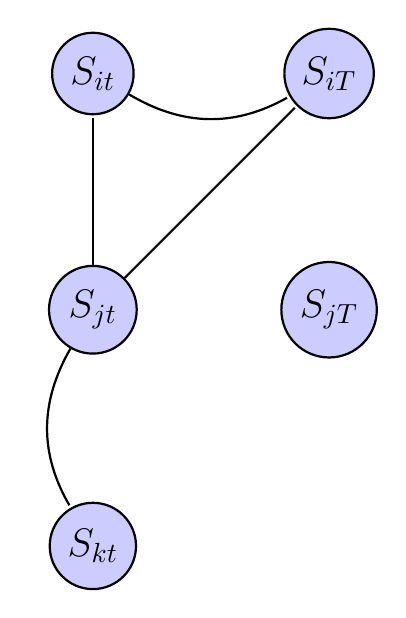
\begin{tikzpicture}[-,-=stealth,shorten >=1pt,auto,node distance=3cm,
  thick,main node/.style={circle,fill=blue!20,draw,font=\sffamily\Large\bfseries}]

  \node[main node] (1) {$S_{it}$};
  \node[main node] (2) [below of=1] {$S_{jt}$};
  \node[main node] (3) [below of=2] {$S_{kt}$};
  \node[main node] (4) [right of=1] {$S_{iT}$};
  \node[main node] (5) [below of=4] {$S_{jT}$};

  \path[every node/.style={font=\sffamily\small}]
    (1) edge [bend right] node [left] {} (4)       
    (2) edge node [right] {} (1)
        edge node {} (4)        
        edge [bend right] node[left] {} (3);
        
\end{tikzpicture}\label{fig:graph1}
%    (3) edge node [right] {} (2)
%        edge [bend right] node[right] {} (4)
%    (4) edge node [left] {} (3)        
%        edge [bend right] node[right] {} (1);

\section{ Markov networks approach}
%%Para analizar cuan relacionado (o no) está un sensor de otro vamos a utilizar
%%el enfoque de la independencia probabilística. Una forma común de representar 
%%distribuciones de probabilidad es mediante independencias condicionales.  
%%Dos eventos $\alpha$ y $\beta$ 
%%son independientes siempre y cuando $P(\alpha | \beta)=P(\alpha)$. Esto significa
%%que saber que $\beta$ ocurre no cambia la probabilidad de ocurrencia de $\alpha$.
%%Una Markov network es un undirected graphical model (grafo no dirigido) que representa
%%la distribución de probabilidad conjunta sobre las variables. Cada nodo en el grafo 
%%representa una variable aleatoria sobre el dominio. Dada
%%una Markov network es posible determinar la independencia condicional de variables 
%%respecto de otras. Una arista entre dos nodos, representa una relación de 
%%dependencia condicional entre esas dos variables. (EXPLICAR E INTRODUCIR 
%%propiedades de M.N: CI pairwise, local, global, CLIQUES, markov blanquet). Esto 
%%permitiría disminuir la complejidad del problema, evitando "analizar" la distribución completa
%%con todas sus variables, concentrándonos sólo en Markov blanquet de la variable.


In order to analyze how related is a sensor respect others, we are going to use the 
probabilistic independence approach. A common way of probability distribution 
representations is conditional independence. Two events $\alpha$ and $\beta$ 
are independent iff $P(\alpha | \beta)=P(\alpha)$. It means if you know
that $\beta$ occurs, it does not change the probability of occurence of $\alpha$.
Markov networs are undirected graphical models which represent a joint probability
distribution over the variables. Each node of the graph is a random variable of the domain
and each edge between nodes represents a dependency conditional relationship
between both variables. Given a Markov network it is able to find the conditional 
independence over the 
variables respect others. It is possible to learn Markov network from data using structure
learning algorithms. We have chosen independence structure learning approach 
\cite{schluter2012survey} for knowledge discovering.

%TODO (EXPLICAR E INTRODUCIR 
%propiedades de M.N: CI pairwise, local, global, CLIQUES, markov blanquet). Esto 
%permitiría disminuir la complejidad del problema, evitando "analizar" la distribución completa
%con todas sus variables, concentrándonos sólo en Markov blanquet de la variable.

\section{ Mutual Information approach}

%ENTROPY
%%La entropía mide la cantidad de información (o incertidumbre) en una variable
%%aleatoria. Siendo X una variable discreta, P(x) su distribución de 
%%probabilidad en X, la entropía H(X) se calcula como

Entropy  measures the amount of information (or uncertainty)
of a random variable. Given X, a discreted random variable and P(x) its probability distribution,
the entropy H(X) is calculated as (\ref{eq:entropy})

\begin{equation}\label{eq:entropy}
H(X)=\sum_{x\in X}P(x) \log P(x)
\end{equation}

If the log base 2 is used, the units are the bit. By definition $H(X) \geq 0$. 
The joint entropy represents the amount of information needed on
average to specify the value of two discrete random variables X and Y which
is given by (\ref{eq:joint-entropy})
%y 
%$H(X) \leq \log_{a}N$, siendo $a$ la base del logaritmo y $N$ la cantidad de variables aleatorias
%JOINT ENTROPY
%La entropía conjunta o joint entropy de dos variables aleatorias discretas X e Y, se 
%calcula de la siguiente manera:

\begin{equation}\label{eq:joint-entropy}
H(X,Y)= \sum_{x\in X}\sum_{y\in Y}P(x,y)\log P(x,y)
\end{equation}


%CONDITIONAL ENTROPY

The conditional entropy indicates how much extra information you
still need to supply on average to communicate Y given that the
other party knows X. Conditional entropy $H (X|Y)$ measures the amount of uncertainty in
X after we know the value of Y (on average):
$H(Y|X)=H(X,Y)-H(X)$

\begin{equation}
H(Y|X)= \sum_{x\in X}\sum_{y\in Y}P(x,y)\log P(y|x)
\end{equation}

%\begin{equation}
%H(Y|X)= \sum_{x\in X}\sum_{y\in Y}P(x,y)\log\frac{ P(x)}{P(x,y)}
%\end{equation}
%MUTUAL INFORMATION
Mutual information measures the information that X and Y share:
it measures how much knowing one of these variables reduces uncertainty
about the other.
%
%Una medida/forma de comparar cuan "relacionadas" estarían dos variables
%es mutual information. \textit{Mutual information} $I(X,Y)$ mide como 
%se reduce la incertidumbre en X al conocer Y.

\begin{equation}
I(X,Y)= \sum_{x\in X}\sum_{y\in Y}P(x,y)\frac{\log P(x,y)}{P(x)P(y)}
\end{equation}

where p(x,y) is the joint probability distribution function of X and Y, 
and p(x) and p(y) are the marginal probability distribution functions of X 
and Y respectively. It is the marginal additional information someone, 
analyzing X ,
gains from knowing Y.
Moreover, $I(X,Y)$ is symetric and non-negative.
 $I(X,Y)=I(Y,X) $. If $I(X,Y)=0$, then X and Y are independent.
 
 
We analyze the conditional entropy of the sensor and their relationships in a 
present time $t$ and a future time $T$ in order to answer:

1) How much reduces the entropy of $H(S_{iT}|S_{it})$ which indicates
how much information gives  $S_{iT}$ given that we have $S_{it}$

2) How much information gives a neighbor $S_{jt}$, calculating $H(S_{iT}|S_{it},S_{jt})$

%1) La entropía de $S_{iT}$ dado $S_{it}$ se refleja como $H(S_{iT}|S_{it})$, que 
%significa cuanta información extra requiere  $S_{iT}$ dado que tiene/sabe $S_{it}$
%¿Cuánta información me otorga $S_{iT}$ dado que se $S_{it}$?
%2) Por otra parte, nos interesa saber cuanta información me otorga agregar a un vecino
%$S_{jt}$, y se refleja en la entropía $H(S_{iT}|S_{it},S_{jt})$


\section{Experimental setup}

Se procedera a explicar las caracteristicas del origen de los datos en \ref{dataset-agrarias} y
su posterior procesamiento en \ref{preproc} (discretizacion, consideracion temporal) para dar 
origen a otros datasets, que serviran como entrada para el aprendizaje de estructura de markov 
y para el analisis de mutual info. En \ref{sec:mn} se presenta la configuracion utilizada para 
el aprendizaje de estructuras. Por ultimo se desglosa los resultados de mutual info.

\subsection{Data source}\label{dataset-agrarias}
%%
%%Un dataset de temperaturas nos fue facilitado gracias a un proyecto de 
%%investigaci\'{o}n\cite{pid-fca-uncu-dataset}. Seis data loggers 
%%LOGTAG\cite{logtag-datalogger} fueron posicionados a distintas alturas, 
%%como se ve en la Tabla \ref{tabla-sensores}. Son seis variables que 
%%representan sensores
%%de temperatura ubicados en la misma posición $(x,y)$ pero variando 
%%su altura (componente $z$). Los datos fueron adquiridos entre el 21/07/2012 
%%y el 26/07/2012
%%en una semana de heladas con un intervalo de muestreo de 1 minuto. 
%%Por cada sensor, hay unos 7330 datapoints.
%%Six data loggers 

Six temperature sensor\cite{logtag-datalogger} from a research project \cite{pid-fca-uncu-dataset}
where placed at different heights, as we can see on table  \ref{tabla-sensores}.
The sampling interval was set to a minute.
They represent six temperature variables located in the same
$(x,y)$ position varing their height. 
The data was acquiered between 07/21/2012 and 07/26/2012,
a week with frost events.
For each sensor there are 7330 datapoints.


\begin{table}[h]
\begin{center}
\begin{tabular}{ l | c | r }
  Temperature sensor & Sensor at time t & Sensor at t + T \\ \hline
  ground level & $S_1$  & $S_7$ \\
  40 cm height & $S_2$   & $S_8$  \\  %antes S_0_4
  75cm height & $S_3$   & $S_9$ \\   %antes S_0_75
  1.5m height & $S_4$   & $S_{10}$ \\  %antes S_1_5
  2m height & $S_5$     & $S_{11}$ \\  %antes S_2
  3m height & $S_6$    & $S_{12}$ \\   %antes S_3
\end{tabular}
\caption{Variables of interest}
\end{center}
\end{table}\label{tabla-sensores}

\subsection{Pre-processing}\label{preproc}

%%\subsubsection{Discretization of sensor values}
%%
%%Se fija un número $k$ de bins o \emph{cute-point} y luego se calcula 
%%el ancho $h$ requerido teniendo en cuenta que $k=\frac{max(x)-min(x)}{h}$, 
%%logrando intervalos del mismo ancho. Se eligió un k=9, para contar con 8 
%%intervalos de temperatura. La temperatura mínima del dataset es -9.8 y la 
%%máxima 26.8.\\

The continuous temperature data is ranging from a minimum -9.8\degree C to 26.8\degree C.
It was discretized with eight intervals with the same width.
 
For the temporal discretization, three options of time displacement interval were chosen:
6, 8 and 12 hours; which were labeled with  T\_1, T\_2 y T\_3 respectively.

%
%\subsubsection{Temporal dimension}
%
%Se discretizó los intervalos temporales eligiendo como intervalos de interés a períodos 
%futuros de 6, 8 y 12 hs, etiquetados como T\_1, T\_2 y T\_3 respectivamente.

\subsubsection{Dataset design}

Para tomar en cuenta el valor de la variable $S_{i}$
en un tiempo $T$ posterior, se diseño dos tipos de datasets que pasaré a explicar.

%\todo{el siguiente dataset no fue usado para analisis x lo q no ira en el poster}

\begin{itemize}

\item [ESTE NO VA A L POSTER] Para analizar la relación de todas las variables $S_{it}$ en $t=t_{0}$,
 versus la predicción de alguna de ellas $S_{kT}$, $i \neq k$, en un $t=T$,, 
donde $i=1..N$ y $N$ el número total de sensores.
Se construyó un dataset cuyas columnas concatenan las variables de la siguiente manera:
Una columna para cada $S_{it}$ (total $N$ columnas) y una columna $S_{kT}$.

\item For analyzing the relationship between the variables $S_{it}$ in $t=t_{0}$, where $i=1..N$ and 
 $N$ is the total number of sensors, versus the prediction of $S_{iT}$ in $t=T$,a dataset was built whose
columns concatenate the variables as follow: one column per each $S_{it}$  and then 
one column per each $S_{iT}$.

\end{itemize}

El número total de datasets resultantes está definido por ( $N$ + 1 ) * $T$. 
Dado que tomaremos 3 períodos futuros, T $\in$ (6,8,12), y $N=6$ para nuestro caso,
contamos con 21 datasets generados.


\subsubsection{Aprendizaje de estructuras: setup} \label{sec:mn}

The setup of structured learning is listed below on Table \ref{sl-algorithm}. 
The first column is the algorithm used ("SL slgorithm"), the second the test
used to calculated if two variables are independent, and the third is the 
threshold used for the test.

%%Grow-Shrink Markov Network (GSMN) \\
%%HHC-MN \\
%%IBMAP \\
\todo[inline]{Agregar una intro a cada uno de ellos}
\begin{table}[h]
\begin{center}
\caption{Setup para aprendizaje de estructuras}
\begin{tabular}{| l | c | r |}
\hline
  SL algorithm & Test & Threshold  \\ \hline \hline
  HHC-MN  \cite{schluter2014ibmap} & $G^2$ & 0.001, 0.01, 0.05 \\ \hline
  GSMN \cite{bromberg2009efficient} &$G^2$ & 0.001, 0.01, 0.05 \\ \hline  
  PC \cite{spirtes2000causation}&$G^2$ & 0.001, 0.01, 0.05  \\  \hline
  IBMAP-HC \cite{schluter2014ibmap} & bayesian test & 0.5  \\  \hline
\end{tabular} 
\end{center}
\end{table}\label{sl-algorithm}

\subsection{Resultados Markov networks}

Las estructuras resultantes para los algoritmos pc, gsmn, hhc 
se encuentran en scripts/structured-learning/output/structures,
y para ibmaph en scripts/structured-learning/output-ibmaph/structures.
Los archivos que guardan las estructuras son extensiones .ugraph.
La nomenclatura a utilizar es la indicada en la Tabla \ref{tabla-sensores}

The Figure \ref{fig:T3-result} shows the result of apply OR-operand 
(counting all edges) between all
the Adjacency matrix obtained from the structured learning algorithms with 
the following setup: threshold 0.001, except IBMAPH with 0.5, and T = 3 (12 hs).
The columns and rows show the variable number, for example 1 is $S1$, which 
are listed on Table \ref{tabla-sensores}. We can see that still with a big confidence interval
remains dependencies between the variables. The relationships between one sensor with its next-door neighbor,
which is located over or below itself, reflects the typical thermodinamic behavior 
because one layer of air is related with other. 
Edges between $S_1$ and $S_5$ explain where the inversion layer is located. 
The inversion layer is the division between the cool air and heat air.

\begin{figure}\label{fig:T3-result}
\includegraphics[scale=0.75]{T3-summarize.png}
\caption{----}
\end{figure}

En el siguiente enlace de gdrive contiene las tablas como la de arriba
\url{https://docs.google.com/spreadsheets/d/16cIB4ZQ2kGtz6VOBqyA9paCYtCYshQuPt7_hV0eqDxs/edit?usp=sharing}

%INTENTO VISUALIZADOR DE TABLA
%%\begin{table}[h]
%%\begin{center}
%%\begin{tabular}{ l c r }
%% 
%% & $S_1$ & $S_2$ &$S_3$ & $S_4$ & $S_5$ & $S_5$ & $S_6$ & $S_7$ & $S_8$ & $S_9$ & $S_{10}$ & $S_{11}$ & $S_{12}$  \\ \hline
%% $S_1$& $S_1$ & $S_2$ &$S_3$ & $S_4$ & $S_5$ & $S_5$ & $S_6$ & $S_7$ & $S_8$ & $S_9$ & $S_{10}$ & $S_{11}$ & $S_{12}$&  \\ \hline
%% & $S_1$ & $S_2$ &$S_3$ & $S_4$ & $S_5$ & $S_5$ & $S_6$ & $S_7$ & $S_8$ & $S_9$ & $S_{10}$ & $S_{11}$ & $S_{12}$&  \\ \hline
%% & $S_1$ & $S_2$ &$S_3$ & $S_4$ & $S_5$ & $S_5$ & $S_6$ & $S_7$ & $S_8$ & $S_9$ & $S_{10}$ & $S_{11}$ & $S_{12}$ & \\ \hline
%% & $S_1$ & $S_2$ &$S_3$ & $S_4$ & $S_5$ & $S_5$ & $S_6$ & $S_7$ & $S_8$ & $S_9$ & $S_{10}$ & $S_{11}$ & $S_{12}$ & \\ \hline
%% & $S_1$ & $S_2$ &$S_3$ & $S_4$ & $S_5$ & $S_5$ & $S_6$ & $S_7$ & $S_8$ & $S_9$ & $S_{10}$ & $S_{11}$ & $S_{12}$ & \\ \hline
%% & $S_1$ & $S_2$ &$S_3$ & $S_4$ & $S_5$ & $S_5$ & $S_6$ & $S_7$ & $S_8$ & $S_9$ & $S_{10}$ & $S_{11}$ & $S_{12}$ & \\ \hline
%% & $S_1$ & $S_2$ &$S_3$ & $S_4$ & $S_5$ & $S_5$ & $S_6$ & $S_7$ & $S_8$ & $S_9$ & $S_{10}$ & $S_{11}$ & $S_{12}$ & \\ \hline
%%\end{tabular}
%%\caption{Variables de inter\'{e}s}
%%\end{center}
%%\end{table}\label{tabla-sensores}

%INTENTO VISUALIZADOR GRAFO TIKZ
%%\begin{tikzpicture}[-,-=stealth,shorten >=1pt,auto,node distance=3cm,
%%  thick,main node/.style={circle,fill=blue!20,draw,font=\sffamily\Large\bfseries}]
%%
%%  \node[main node] (1) {$S_1$};
%%  \node[main node] (2) [below of=1] {$S_2$};
%%  \node[main node] (3) [below of=2] {$S_3$};
%%  \node[main node] (4) [below of=3] {$S_4$};
%%  \node[main node] (5) [below of=4] {$S_5$};
%%  \node[main node] (6) [below of=5] {$S_6$};
%%  \node[main node] (7) [right of=1] {$S_7$};
%%  \node[main node] (8) [below of=7] {$S_8$};
%%  \node[main node] (9) [below of=8] {$S_9$};
%%  \node[main node] (10) [below of=9] {$S_{10}$};
%%  \node[main node] (11) [below of=10] {$S_{11}$};
%%  \node[main node] (12) [below of=11] {$S_{12}$};
%%
%%  \path[every node/.style={font=\sffamily\small}]
%%    (1) edge [bend right] node [left] {} (4)       
%%    (2) edge node [right] {} (1)
%%        edge node {} (4)        
%%        edge [bend right] node[left] {} (3)
%%    (3) edge node [right] {} (2)
%%        edge [bend right] node[right] {} (4)
%%    (4) edge node [left] {} (3)        
%%        edge [bend right] node[right] {} (1);
%%        
%%\end{tikzpicture}

%Issue #5 NEW Resolve  Workflow  More  Edit
%Sección de entropia (Renglon 177 del PDF) - falta motivación
%Facundo Bromberg avatarFacundo Bromberg created an issue 2014-07-28
%Ana, será muy util explicar porque mutual information es una medida adecuada, y que resuelve/mejora respecto a las estructuras. Esto lo charlamos varias veces y no veo que haya sido incorporado en el texto. En pocas palabras, para recordarte, era algo respecto que los tests de independencia no repiortan explicitamente el poder predictivo, mientras que MI sí. Explicar como poder predictivo equivale a pico en la distribución de probabilidad, y como eso agregado para todos los casos resulta en MI.
%Comments (1)
%Facundo Bromberg
%¿Como es que mutual information ayuda en confirmar/rechazar la hipotesis de que los sitios vecinos aumentan el poder predictivo?


\section{Resultados mutual information}

Los cálculos de mutual information se encuentran implementados
en el archivo mutual.information.R, método run.experiment.cond.entropy.
Se procedió a calcular los siguiente:

1) La entropía de $S_{iT}$ dado $S_{it}$ se refleja como $H(S_{iT}|S_{it})$, que 
significa cuanta información extra requiere  $S_{iT}$ dado que tiene/sabe $S_{it}$.
¿En cuánto me ayuda a disminuir la incertidumbre de $S_{iT}$ 
saber $S_{it}$?

2) Por otra parte, nos interesa saber cuanta información me otorga agregar a un vecino
$S_{jt}$, y se refleja en la entropía $H(S_{iT}|S_{it},S_{jt})$

Los cálculos son en base e, en consecuencia el resultado son nats (no bits).

En la vector de resultados de $H(S_{iT}|S_{it})$ cada posición i guarda el valor de uno
de los cálculos. En la matriz de resultados de $H(S_{iT}|S_{it},S_{jt})$, un resultado 
en la posición (i,j) siendo i la fila y j la columna; por ej, la fila de s\_2 y 
columna  s3\_t guarda el 
resultado de calcular $H(S_{2T}|S_{2t},S_{3t})$.

Each cell (i,j), where $i$ is the row
and $j$ the column,
 of the matrix stores one result of $H(S_{iT}|S_{it},S_{jt})$. 
 For example the row 2 ($S_2$) and column $S_3$ stores the result of calculate
$H(S_{2T}|S_{2t},S_{3t})$.

\begin{verbatim}
> run.experiment.cond.entropy()
[1] "/home/usuario/phd/heladas/frost/heladas/scripts/datasets/T_1_b_8.csv"
CALCULO DE H(X)  X=S_T 
   value
s1  8.69
s2  8.74
s3  8.76
s4  8.77
s5  8.77
s6  8.78
CALCULO DE H(X | Y) donde:   X=S_T     Y=S_t 
   value
s1  1.65
s2  1.56
s3  1.52
s4  1.50
s5  1.49
s6  1.48
CALCULO DE H(X | Y,Z) donde:   X=Si_T     Y=Si_t   Z=Sj_t
     s1   s2   s3   s4   s5   s6
s1 1.65 1.50 1.45 1.49 1.46 1.48
s2 1.41 1.56 1.50 1.48 1.43 1.49
s3 1.34 1.47 1.52 1.47 1.43 1.46
s4 1.33 1.43 1.45 1.50 1.43 1.43
s5 1.32 1.39 1.42 1.44 1.49 1.40
s6 1.32 1.42 1.42 1.41 1.38 1.48
MUTUAL INFO I(X,Z|Y) donde:   X=Si_T     Y=Si_t   Z=Sj_t
     s1   s2   s3   s4   s5   s6
s1 0.00 0.15 0.19 0.16 0.18 0.17
s2 0.16 0.00 0.06 0.08 0.14 0.07
s3 0.18 0.05 0.00 0.05 0.09 0.05
s4 0.17 0.07 0.05 0.00 0.07 0.07
s5 0.17 0.11 0.07 0.05 0.00 0.09
s6 0.16 0.06 0.06 0.07 0.10 0.00
METRICA razon o division del 3ro con el 2do 
     s1   s2   s3   s4   s5   s6
s1 1.00 0.91 0.88 0.90 0.89 0.90
s2 0.90 1.00 0.96 0.95 0.91 0.95
s3 0.88 0.97 1.00 0.97 0.94 0.96
s4 0.88 0.95 0.97 1.00 0.95 0.95
s5 0.88 0.93 0.95 0.96 1.00 0.94
s6 0.89 0.96 0.96 0.96 0.93 1.00
porcentaje de reducción de la entropía 
     s1   s2   s3   s4   s5   s6
s1 0.00 0.09 0.12 0.10 0.11 0.10
s2 0.10 0.00 0.04 0.05 0.09 0.05
s3 0.12 0.03 0.00 0.03 0.06 0.04
s4 0.12 0.05 0.03 0.00 0.05 0.05
s5 0.12 0.07 0.05 0.04 0.00 0.06
s6 0.11 0.04 0.04 0.04 0.07 0.00
[1] "/home/usuario/phd/heladas/frost/heladas/scripts/datasets/T_2_b_8.csv"
CALCULO DE H(X)  X=S_T 
   value
s1  8.67
s2  8.72
s3  8.74
s4  8.75
s5  8.75
s6  8.76
CALCULO DE H(X | Y) donde:   X=S_T     Y=S_t 
   value
s1  1.58
s2  1.45
s3  1.43
s4  1.35
s5  1.40
s6  1.36
CALCULO DE H(X | Y,Z) donde:   X=Si_T     Y=Si_t   Z=Sj_t
     s1   s2   s3   s4   s5   s6
s1 1.58 1.41 1.38 1.40 1.39 1.39
s2 1.36 1.45 1.39 1.38 1.37 1.39
s3 1.30 1.37 1.43 1.34 1.34 1.34
s4 1.25 1.29 1.29 1.35 1.30 1.29
s5 1.26 1.29 1.30 1.33 1.40 1.33
s6 1.23 1.29 1.28 1.29 1.29 1.36
MUTUAL INFO I(X,Z|Y) donde:   X=Si_T     Y=Si_t   Z=Sj_t
     s1   s2   s3   s4   s5   s6
s1 0.00 0.17 0.20 0.18 0.19 0.19
s2 0.09 0.00 0.06 0.08 0.08 0.06
s3 0.12 0.06 0.00 0.08 0.09 0.08
s4 0.10 0.06 0.06 0.00 0.05 0.07
s5 0.14 0.11 0.10 0.07 0.00 0.07
s6 0.13 0.07 0.07 0.06 0.07 0.00
METRICA razon o division del 3ro con el 2do 
     s1   s2   s3   s4   s5   s6
s1 1.00 0.89 0.87 0.89 0.88 0.88
s2 0.94 1.00 0.96 0.95 0.94 0.96
s3 0.91 0.96 1.00 0.94 0.94 0.94
s4 0.92 0.95 0.96 1.00 0.96 0.95
s5 0.90 0.92 0.93 0.95 1.00 0.95
s6 0.91 0.95 0.95 0.95 0.95 1.00
porcentaje de reducción de la entropía 
     s1   s2   s3   s4   s5   s6
s1 0.00 0.11 0.13 0.11 0.12 0.12
s2 0.06 0.00 0.04 0.05 0.06 0.04
s3 0.09 0.04 0.00 0.06 0.06 0.06
s4 0.08 0.05 0.04 0.00 0.04 0.05
s5 0.10 0.08 0.07 0.05 0.00 0.05
s6 0.09 0.05 0.05 0.05 0.05 0.00
[1] "/home/usuario/phd/heladas/frost/heladas/scripts/datasets/T_3_b_8.csv"
CALCULO DE H(X)  X=S_T 
   value
s1  8.63
s2  8.69
s3  8.70
s4  8.71
s5  8.72
s6  8.73
CALCULO DE H(X | Y) donde:   X=S_T     Y=S_t 
   value
s1  1.40
s2  1.37
s3  1.31
s4  1.33
s5  1.32
s6  1.24
CALCULO DE H(X | Y,Z) donde:   X=Si_T     Y=Si_t   Z=Sj_t
     s1   s2   s3   s4   s5   s6
s1 1.40 1.31 1.29 1.29 1.29 1.29
s2 1.28 1.37 1.33 1.32 1.31 1.31
s3 1.19 1.27 1.31 1.28 1.25 1.24
s4 1.21 1.26 1.27 1.33 1.28 1.26
s5 1.22 1.25 1.26 1.28 1.32 1.26
s6 1.15 1.19 1.17 1.18 1.19 1.24
MUTUAL INFO I(X,Z|Y) donde:   X=Si_T     Y=Si_t   Z=Sj_t
     s1   s2   s3   s4   s5   s6
s1 0.00 0.09 0.11 0.11 0.12 0.12
s2 0.09 0.00 0.04 0.06 0.06 0.06
s3 0.12 0.04 0.00 0.03 0.06 0.07
s4 0.11 0.07 0.05 0.00 0.05 0.07
s5 0.09 0.07 0.06 0.04 0.00 0.05
s6 0.09 0.05 0.07 0.06 0.05 0.00
METRICA razon o division del 3ro con el 2do 
     s1   s2   s3   s4   s5   s6
s1 1.00 0.93 0.92 0.92 0.92 0.92
s2 0.94 1.00 0.97 0.96 0.96 0.96
s3 0.91 0.97 1.00 0.98 0.95 0.95
s4 0.91 0.95 0.96 1.00 0.96 0.95
s5 0.93 0.95 0.96 0.97 1.00 0.96
s6 0.92 0.96 0.94 0.95 0.96 1.00
porcentaje de reducción de la entropía 
     s1   s2   s3   s4   s5   s6
s1 0.00 0.07 0.08 0.08 0.08 0.08
s2 0.06 0.00 0.03 0.04 0.04 0.04
s3 0.09 0.03 0.00 0.02 0.05 0.05
s4 0.09 0.05 0.04 0.00 0.04 0.05
s5 0.07 0.05 0.04 0.03 0.00 0.04
s6 0.08 0.04 0.06 0.05 0.04 0.00
\end{verbatim}
\section{Open issues}

\begin{itemize}
\item Complete interpretation with an expert of the markov networks: could they help 
to understand the frost phenomenon?
\item Setup of the prediction model: input and output variables
\item Discretization of continuous features: sensor values and time
\item How to infer the best sensor location in order to optimize the prediction
and the number of sensor needed.
\end{itemize}

\bibliographystyle{plain} %TODO <--- chequear que tome este estilo de bibliografía
\bibliography{references}



\section*{Appendix: Otros issues}

\begin{enumerate}
\item Se puede optimizar la ubicación de los sensores en una finca 
para maximizar el poder de los algoritmos predictivos
(Kriging, Conditional Random Fields). 
\item \emph{Discretización}: Existen otros criterios para discretizar como el criterio 
de Sturge que computa $k=\log_2n+1 $, donde $n$ es el número total de datapoints 
(instancias de dato, hechos, filas). Hasta la versión (commit) 
\todo[inline]{NOMBRAR LA VERSION} 
no investigué adecuadamente como discretizar las 
variables y elegí probar con distintos números de intervalos k. Un método de 
discretización interesante que encontré fue Ameva, whose objective is to 
maximize the dependence between the intervals that divide the values of an 
attribute and the classes to which they belong, providing at the same time 
the minimum number of intervals. En R, la librería discretizacion lo trae implementado.
Para usarlo, llamar al método disc.Topdown(data,method=3). La ventaja de AMEVA es que 
uno puede desligarse de indicarle el valor de k o h al algoritmo, lo calcula solo.
mas info: unas slides introductorias pero mencionan todos los aspectos vinculados a 
discretización 
(SLIDES http://stat.skku.ac.kr/myhuh/homepage/specialLectures/SDULecture.pdf)
Recopilaci\'{o}n de info interesante sobre mutual information y su implementación
en R.\\

\begin{verbatim}
 RECOMENDABLE!!! --> Entropy-Based Inference using R and the np Package: 
 A Primer http://socserv.mcmaster.ca/racine/entropy_np.pdf

 OTRO DOC más info en "Inequality, Entropy and Goodness of Fit"
 http://personal.lse.ac.uk/BANDYOPS/GoF1.pdf
 UNAS SLIDES ACLARATORIAS http://www.unc.edu/~maguilar/metrics/Myslides_trans2.pdf
\end{verbatim}

\end{enumerate}

\end{document}
